\subsection {Session 8, Exercise 7}
\label{8f7}

\lineparagraph {Exercise}

Give a Karp-reduction from $PARTITION$ to $SUBSETSUM$.

\lineparagraph {Solution}

\begin{center}
    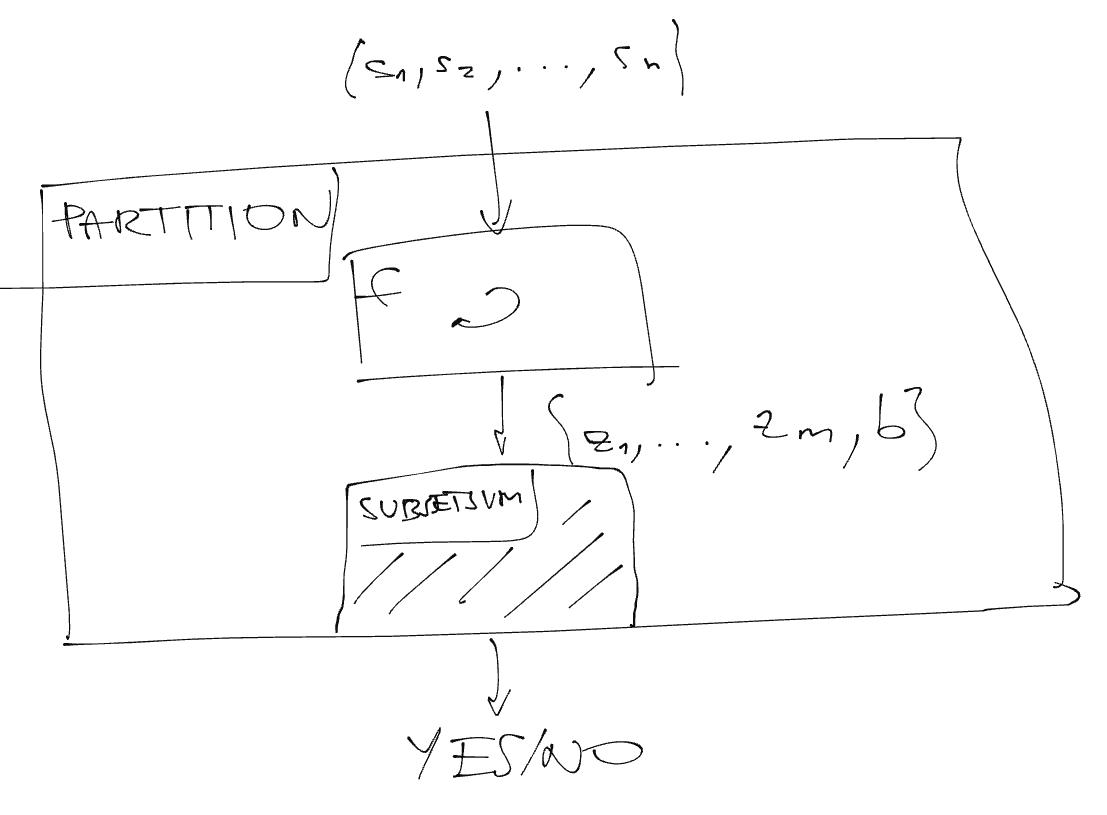
\includegraphics[width=\linewidth]{./08/07/partition_karp_subsetsum.png}
\end{center}

\begin{itemize}
    \item So we need to solve $PARTITION$ uing $SUBSETSUM$.
    \item $PARTITION$ tells us whether or not we separtate our numbers into two sets for which their sum is equal.
    \item $SUBSETSUM$ tells us whether we can find a subset of numbers, for which their sum is a specific number.
    \item In $PARTITION$ we can quickly figure out what the sum of the two sets should be, by just summing up all the input numbers and dividing them by $2$.
    \item If the sum is an odd number, then the answer is immediately no. There is no way to divide those numbers equally, since if the sum of the two equal parts would be some number $a=a$, then the total sum should be $2a$, which is even.
    \item So if the sum is odd, we need to make $SUBSETSUM$ return a $NO$ answer, this can be done by creating an artificial input: $\{2,2\}$ and $b=1$. 
    \item There is no way to select a subset from $\{2,2\}$, for which the sum of those numbers would be equal to $1$, so this definitely results in a $NO$ answer.
    \item In the even case, when we divide by $2$ we get what the sum of one of the subsets should be, let's call this $a$.
    \item We can give the original input numbers to $SUBSETSUM$ and this $a$ number, which will tell us if it can find a subset for which the sum is exactly this $a$. Since the total sum was $2a$, this also means that the remaining numbers will also add up to $a$ as well, making this a partition.
    \item If the original input is even, but cannot be partitioned, then there is no way the $SUBSETSUM$ will find a subset of these numbers for which, their sum is $a$. If we indirectly assume that it did, then that would mean that the remaining numbers will also add up to $a$, so this is a partition, which is a contradiction.
    \item To calculate the total sum of these $n$ numbers and divide by $2$, we have used up polynomial time, so the transformation function is polynomial as well.
\end{itemize}